\newpage
\subsection{Caso d'uso UC14: Amministrazione applicazione web}
\label{UC14}
\begin{figure}[ht]
	\centering
	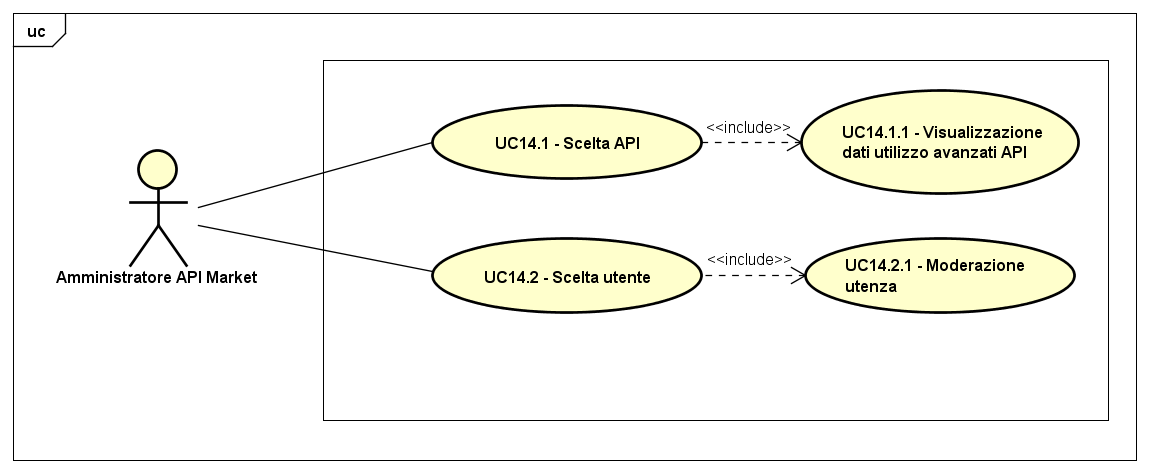
\includegraphics[scale=0.45]{UML/UC14.png}
	\caption{UC14: Amministrazione applicazione web}
\end{figure}

\begin{longtable}{ l | p{11cm}}
	\hline
	\rowcolor{Gray}
	\multicolumn{2}{c}{UC14: Amministrazione applicazione web} \\
	\hline
	\textbf{Attori} & Amministratore API Market \\
	\textbf{Descrizione} & L'attore amministra l'applicazione web e/o consulta i dati di utilizzo avanzati \\
	\textbf{Pre-Condizioni} & L'attore si trova nella schermata iniziale dell'applicazione web \\
	\textbf{Post-Condizioni} & L'attore ha amministrato l'applicazione web e/o ha consultato i dati di utilizzo avanzati \\
	\textbf{Scenario Principale} & 
	\begin{enumerate*}[label=(\arabic*.),itemjoin={\newline}]
		\item L'attore può consultare i dati di utilizzo avanzati (UC14.1)
		\item L'attore può moderare l'utenza (UC14.2)
	\end{enumerate*}\\
\end{longtable}

\newpage
\subsubsection{Caso d'uso UC14.1: Visualizzazione dati di utilizzo avanzati}
\label{UC14_1}
\begin{figure}[ht]
	\centering
	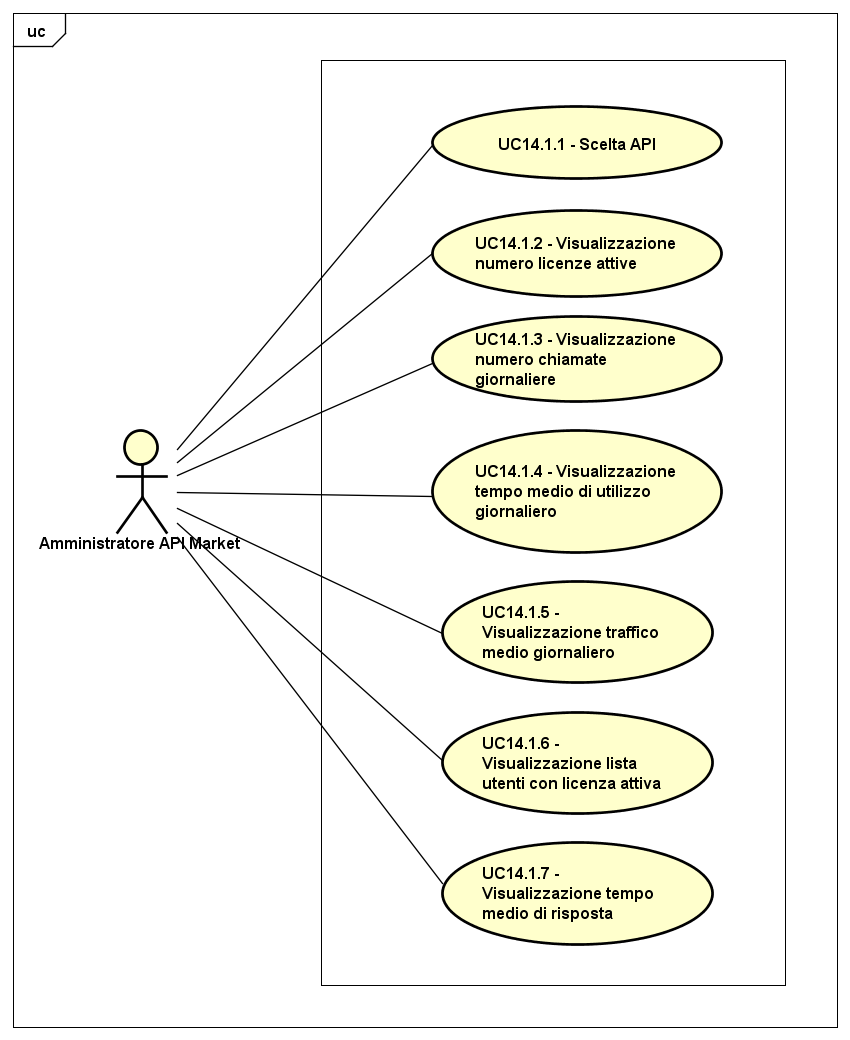
\includegraphics[scale=0.45]{UML/UC14_1.png}
	\caption{UC14.1: Visualizzazione dati di utilizzo avanzati}
\end{figure}

\begin{minipage}{\linewidth}
	\begin{tabular}{ l | p{11cm}}
		\hline
		\rowcolor{Gray}
		\multicolumn{2}{c}{UC14.1 - Visualizzazione dati di utilizzo avanzati} \\
		\hline
		\textbf{Attori} &  Amministratore API Market \\
		\textbf{Descrizione} & L'attore sceglie una API e ne visualizza i dati di utilizzo avanzati \\
		\textbf{Pre-Condizioni} & L'attore si trova nella schermata relativa all'amministrazione dell'applicazione web \\
		\textbf{Post-Condizioni} & L'attore ha scelto una API e ne ha visualizzato i dati di utilizzo avanzati \\
		\textbf{Scenario Principale} & 
		\begin{enumerate*}[label=(\arabic*.),itemjoin={\newline}]
			\item L'attore può scegliere una API di cui visualizzare i dati di utilizzo avanzati (UC14.1.1)
			\item L'attore può visualizzare il numero di licenze attive dell'API scelta (UC14.1.2)
			\item L'attore può visualizzare il numero di chiamate giornaliere effettuate all'API scelta (UC14.1.3)
			\item L'attore può visualizzare il tempo medio di utilizzo giornaliero dell'API scelta (UC14.1.4)
			\item L'attore può visualizzare il traffico medio giornaliero dell'API scelta (UC14.1.5)
			\item L'attore può visualizzare la lista degli utenti con una licenza attiva per l'API scelta (UC14.1.6)
			\item L'attore può visualizzare il tempo medio di risposta dell'API scelta (UC14.1.7)
		\end{enumerate*}\\
	\end{tabular}
\end{minipage}

\paragraph{Caso d'uso UC14.1.1: Scelta API}
\label{UC14_1_1}

\begin{minipage}{\linewidth}
	\begin{tabular}{ l | p{11cm}}
		\hline
		\rowcolor{Gray}
		\multicolumn{2}{c}{UC14.1.1 - Scelta API} \\
		\hline
		\textbf{Attori} & Amministratore API Market \\
		\textbf{Descrizione} & L'attore sceglie una API su cui visualizzare i dati di utilizzo avanzati \\
		\textbf{Pre-Condizioni} & L'attore si trova nella schermata relativa alla visualizzazione dei dati di utilizzo avanzati \\
		\textbf{Post-Condizioni} & L'attore ha scelto una API su cui visualizzare i dati di utilizzo avanzati \\
		\textbf{Scenario Principale} & 
		\begin{enumerate*}[label=(\arabic*.),itemjoin={\newline}]
			\item L'attore può scegliere una API su cui visualizzare i dati di utilizzo avanzati
		\end{enumerate*}\\
	\end{tabular}
\end{minipage}

\paragraph{Caso d'uso UC14.1.2: Visualizzazione numero licenze attive}
\label{UC14_1_2}

\begin{minipage}{\linewidth}
	\begin{tabular}{ l | p{11cm}}
		\hline
		\rowcolor{Gray}
		\multicolumn{2}{c}{UC14.1.2 - Visualizzazione numero licenze attive} \\
		\hline
		\textbf{Attori} & Amministratore API Market \\
		\textbf{Descrizione} & L'attore visualizza il numero di licenze attive per l'API scelta \\
		\textbf{Pre-Condizioni} & L'attore si trova nella schermata di visualizzazione dati di utilizzo API avanzati ed ha scelto una API \\
		\textbf{Post-Condizioni} & L'attore ha visualizzato il numero di licenze attive per l'API scelta \\
		\textbf{Scenario Principale} & 
		\begin{enumerate*}[label=(\arabic*.),itemjoin={\newline}]
			\item L'attore può visualizzare il numero di licenze attive per l'API scelta
		\end{enumerate*}\\
	\end{tabular}
\end{minipage}

\paragraph{Caso d'uso UC14.1.3: Visualizzazione numero chiamate giornaliere}
\label{UC14_1_3}

\begin{minipage}{\linewidth}
	\begin{tabular}{ l | p{11cm}}
		\hline
		\rowcolor{Gray}
		\multicolumn{2}{c}{UC14.1.3 - Visualizzazione numero chiamate giornaliere} \\
		\hline
		\textbf{Attori} & Amministratore API Market \\
		\textbf{Descrizione} & L'attore visualizza il numero di chiamate giornaliere effettuate all'API scelta \\
		\textbf{Pre-Condizioni} & L'attore si trova nella schermata di visualizzazione dati di utilizzo API avanzati ed ha scelto una API \\
		\textbf{Post-Condizioni} & L'attore ha visualizzato il numero di chiamate giornaliere effettuate all'API scelta \\
		\textbf{Scenario Principale} & 
		\begin{enumerate*}[label=(\arabic*.),itemjoin={\newline}]
			\item L'attore può visualizzare il numero di chiamate giornaliere effettuate all'API scelta
		\end{enumerate*}\\
	\end{tabular}
\end{minipage}

\paragraph{Caso d'uso UC14.1.4: Visualizzazione tempo medio di utilizzo giornaliero}
\label{UC14_1_4}

\begin{minipage}{\linewidth}
	\begin{tabular}{ l | p{11cm}}
		\hline
		\rowcolor{Gray}
		\multicolumn{2}{c}{14.1.4 - Visualizzazione tempo medio di utilizzo giornaliero} \\
		\hline
		\textbf{Attori} & Amministratore API Market \\
		\textbf{Descrizione} & L'attore visualizza il tempo medio di utilizzo giornaliero dell'API scelta \\
		\textbf{Pre-Condizioni} & L'attore si trova nella schermata di visualizzazione dati di utilizzo API avanzati ed ha scelto una API \\
		\textbf{Post-Condizioni} & L'attore ha visualizzato il tempo medio di utilizzo giornaliero dell'API scelta \\
		\textbf{Scenario Principale} & 
		\begin{enumerate*}[label=(\arabic*.),itemjoin={\newline}]
			\item L'attore può visualizzare il tempo medio di utilizzo giornaliero dell'API scelta
		\end{enumerate*}\\
	\end{tabular}
\end{minipage}

\paragraph{Caso d'uso UC14.1.5: Visualizzazione traffico medio giornaliero}
\label{UC14_1_5}

\begin{minipage}{\linewidth}
	\begin{tabular}{ l | p{11cm}}
		\hline
		\rowcolor{Gray}
		\multicolumn{2}{c}{UC14.1.5 - Visualizzazione traffico medio giornaliero} \\
		\hline
		\textbf{Attori} & Amministratore API Market \\
		\textbf{Descrizione} & L'attore visualizza il traffico medio giornaliero dell'API scelta \\
		\textbf{Pre-Condizioni} & L'attore si trova nella schermata di visualizzazione dati di utilizzo API avanzati ed ha scelto una API \\
		\textbf{Post-Condizioni} & L'attore ha visualizzato il traffico medio giornaliero dell'API scelta \\
		\textbf{Scenario Principale} & 
		\begin{enumerate*}[label=(\arabic*.),itemjoin={\newline}]
			\item L'attore può visualizzare il traffico medio giornaliero dell'API scelta
		\end{enumerate*}\\
	\end{tabular}
\end{minipage}

\newpage
\paragraph{Caso d'uso UC14.1.6: Visualizzazione utenti con licenza attiva}
\label{UC14_1_6}
\begin{figure}[ht]
	\centering
	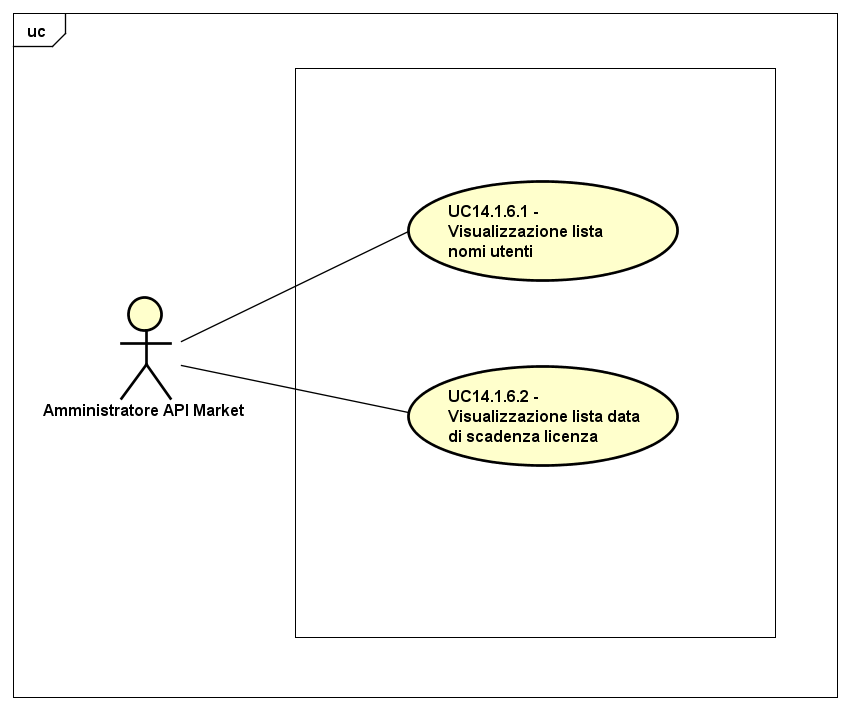
\includegraphics[scale=0.45]{UML/UC14_1_6.png}
	\caption{UC14.1.6: Visualizzazione utenti con licenza attiva}
\end{figure}

\begin{minipage}{\linewidth}
	\begin{tabular}{ l | p{11cm}}
		\hline
		\rowcolor{Gray}
		\multicolumn{2}{c}{UC14.1.6 - Visualizzazione utenti con licenza attiva} \\
		\hline
		\textbf{Attori} & Amministratore API Market \\
		\textbf{Descrizione} & L'attore ha scelto una API e visualizza una lista di utenti con licenze attive per l'API scelta\\
		\textbf{Pre-Condizioni} & L'attore si trova nella schermata di visualizzazione dati di utilizzo API avanzati ed ha scelto una API \\
		\textbf{Post-Condizioni} & L'attore ha visualizzato la lista di utenti con licenze attive per l'API scelta \\
		\textbf{Scenario Principale} & 
		\begin{enumerate*}[label=(\arabic*.),itemjoin={\newline}]
			\item L'attore può visualizzare il nome di ogni utente con licenza attiva per l'API scelta (UC14.1.6.1)
			\item L'attore può visualizzare la data di scadenza della licenza per ogni utente nella lista (UC14.1.6.2)
		\end{enumerate*}\\
	\end{tabular}
\end{minipage}

\subparagraph{Caso d'uso UC14.1.6.1: Visualizzazione lista nomi utenti}
\label{UC14_1_6_1}

\begin{minipage}{\linewidth}
	\begin{tabular}{ l | p{11cm}}
		\hline
		\rowcolor{Gray}
		\multicolumn{2}{c}{UC14.1.6.1 - Visualizzazione lista nomi utenti} \\
		\hline
		\textbf{Attori} & Amministratore API Market \\
		\textbf{Descrizione} & L'attore ha scelto una API e visualizza il nome dell'utente interessato\\
		\textbf{Pre-Condizioni} & L'attore si trova nella schermata di visualizzazione dati di utilizzo API avanzati ed ha scelto una API \\
		\textbf{Post-Condizioni} & L'attore ha visualizzato il nome per ogni utente della lista degli utenti con licenza attiva per l'API scelta \\
		\textbf{Scenario Principale} & 
		\begin{enumerate*}[label=(\arabic*.),itemjoin={\newline}]
			\item L'attore può visualizzare il nome per ogni utente della lista degli utenti con licenza attiva per l'API scelta
		\end{enumerate*}
	\end{tabular}
\end{minipage}

\subparagraph{Caso d'uso UC14.1.6.2: Visualizzazione lista data di scadenza licenza}
\label{UC14_1_6_2}

\begin{minipage}{\linewidth}
	\begin{tabular}{ l | p{11cm}}
		\hline
		\rowcolor{Gray}
		\multicolumn{2}{c}{UC14.1.6.2 -  Visualizzazione lista data di scadenza licenza} \\
		\hline
		\textbf{Attori} & Amministratore API Market \\
		\textbf{Descrizione} & L'attore ha scelto una API e visualizza la data di scadenza per ogni utente della lista degli utenti con licenza attiva per l'API scelta \\
		\textbf{Pre-Condizioni} & L'attore si trova nella schermata di visualizzazione dati di utilizzo API avanzati ed ha scelto una API \\
		\textbf{Post-Condizioni} & L'attore ha visualizzato la data di scadenza per ogni utente della lista degli utenti con licenza attiva per l'API scelta \\
		\textbf{Scenario Principale} & 
		\begin{enumerate*}[label=(\arabic*.),itemjoin={\newline}]
			\item L'attore può visualizzare la data di scadenza per ogni utente della lista degli utenti con licenza attiva per l'API scelta
		\end{enumerate*}
	\end{tabular}
\end{minipage}

\paragraph{Caso d'uso UC14.1.7: Visualizzazione tempo medio di risposta}
\label{UC14_1_7}

\begin{minipage}{\linewidth}
	\begin{tabular}{ l | p{11cm}}
		\hline
		\rowcolor{Gray}
		\multicolumn{2}{c}{UC14.1.7 - Visualizzazione tempo medio di risposta} \\
		\hline
		\textbf{Attori} & Amministratore API Market \\
		\textbf{Descrizione} & L'attore ha scelto una API e visualizza il tempo medio di risposta dell'API scelta \\
		\textbf{Pre-Condizioni} & L'attore si trova nella schermata di visualizzazione dati di utilizzo API avanzati ed ha scelto una API \\
		\textbf{Post-Condizioni} & L'attore ha visualizzato il tempo medio di risposta dell'API scelta \\
		\textbf{Scenario Principale} & 
		\begin{enumerate*}[label=(\arabic*.),itemjoin={\newline}]
			\item L'attore può visualizzare il tempo medio di risposta dell'API scelta
		\end{enumerate*}\\
	\end{tabular}
\end{minipage}

\newpage
\subsubsection{Caso d'uso UC14.2: Moderazione utenza}
\label{UC14_2}
\begin{figure}[ht]
	\centering
	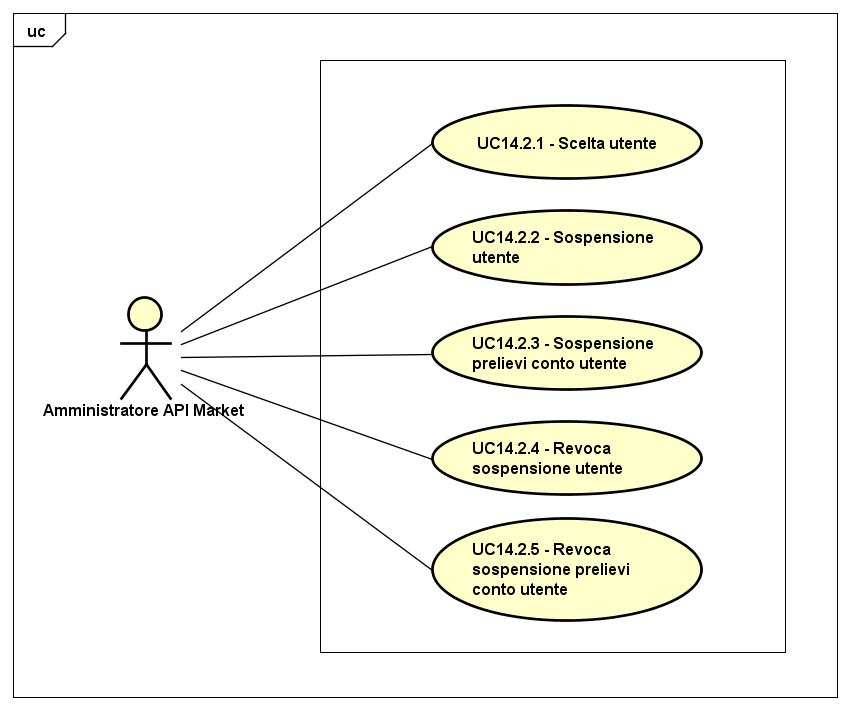
\includegraphics[scale=0.45]{UML/UC14_2.png}
	\caption{UC14.2: Moderazione utenza}
\end{figure}

\begin{minipage}{\linewidth}
	\begin{tabular}{ l | p{11cm}}
		\hline
		\rowcolor{Gray}
		\multicolumn{2}{c}{UC14.2 - Moderazione utenza} \\
		\hline
		\textbf{Attori} &  Amministratore API Market \\
		\textbf{Descrizione} & L'attore attua l'opera di moderazione \\
		\textbf{Pre-Condizioni} & L'attore si trova nella schermata relativa all'amministrazione dell'applicazione web \\
		\textbf{Post-Condizioni} & L'attore ha concluso l'opera di moderazione \\
		\textbf{Scenario Principale} & 
		\begin{enumerate*}[label=(\arabic*.),itemjoin={\newline}]
			\item L'attore può scegliere un utente su cui intervenire (UC14.2.1)
			\item L'attore può sospendere l'utente scelto (UC14.2.2)
			\item L'attore può sospendere i prelievi dell'utente scelto dal rispettivo conto personale (UC14.2.3)
			\item L'attore può revocare la sospensione dell'utente scelto (UC14.2.4)
			\item L'attore può revocare la sospensione dei prelievi dell'utente scelto dal rispettivo conto personale (UC14.2.5)
		\end{enumerate*}\\
		\textbf{Scenari Alternativi} & 
		\begin{enumerate*}[label=(\arabic*.),itemjoin={\newline}]
			\item L'attore riceve un messaggio d'errore informativo (E.g: Scelta dell'utente non valida)
		\end{enumerate*}\\
	\end{tabular}
\end{minipage}

\paragraph{Caso d'uso UC14.2.1: Scelta utente}
\label{UC14_2_1}

\begin{minipage}{\linewidth}
	\begin{tabular}{ l | p{11cm}}
		\hline
		\rowcolor{Gray}
		\multicolumn{2}{c}{UC14.2.1 - Scelta utente} \\
		\hline
		\textbf{Attori} & Amministratore API Market \\
		\textbf{Descrizione} & L'attore sceglie un utente su cui intervenire \\
		\textbf{Pre-Condizioni} & L'attore si trova nella schermata relativa alla moderazione dell'utenza \\
		\textbf{Post-Condizioni} & L'attore ha scelto un utente su cui intervenire \\
		\textbf{Scenario Principale} & 
		\begin{enumerate*}[label=(\arabic*.),itemjoin={\newline}]
			\item L'attore può scegliere un utente su cui intervenire
		\end{enumerate*}\\
	\end{tabular}
\end{minipage}

\newpage
\paragraph{Caso d'uso UC14.2.2: Sospensione utente}
\label{UC14_2_2}
\begin{figure}[ht]
	\centering
	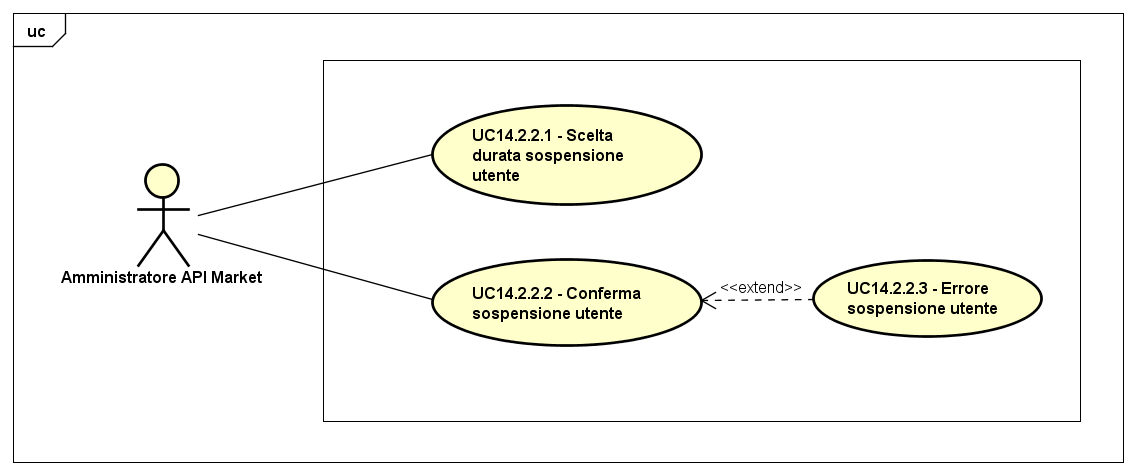
\includegraphics[scale=0.45]{UML/UC14_2_2.png}
	\caption{UC14.2.2: Sospensione utente}
\end{figure}

\begin{minipage}{\linewidth}
	\begin{tabular}{ l | p{11cm}}
		\hline
		\rowcolor{Gray}
		\multicolumn{2}{c}{UC14.2.2 - Sospensione utente} \\
		\hline
		\textbf{Attori} & Amministratore API Market \\
		\textbf{Descrizione} & L'attore sospende l'utente scelto per il numero desiderato di giorni \\
		\textbf{Pre-Condizioni} & L'attore si trova nella schermata relativa alla moderazione dell'utenza ed ha scelto un utente \\
		\textbf{Post-Condizioni} & L'attore ha sospeso l'utente scelto per il numero desiderato di giorni \\
		\textbf{Scenario Principale} & 
		\begin{enumerate*}[label=(\arabic*.),itemjoin={\newline}]
			\item L'attore può inserire la durata in giorni della sospensione dell'utente scelto (UC14.2.2.1)
			\item L'attore può confermare la sospensione dell'utente scelto (UC14.2.2.2)
		\end{enumerate*}\\
		\textbf{Scenari Alternativi} & 
		\begin{enumerate*}[label=(\arabic*.),itemjoin={\newline}]
			\item L'attore può visualizzare un messaggio di errore informativo e la sospensione dell'utente scelto non avviene
		\end{enumerate*}\\
	\end{tabular}
\end{minipage}

\subparagraph{Caso d'uso UC14.2.2.1: Scelta durata sospensione utente}
\label{UC14_2_2_1}

\begin{minipage}{\linewidth}
	\begin{tabular}{ l | p{11cm}}
		\hline
		\rowcolor{Gray}
		\multicolumn{2}{c}{UC14.2.2.1 - Scelta durata sospensione utente} \\
		\hline
		\textbf{Attori} & Amministratore API Market \\
		\textbf{Descrizione} & L'attore inserisce la durata in giorni della sospensione dell'utente scelto, oppure lascia il valore di default \\
		\textbf{Pre-Condizioni} & L'attore si trova nella schermata relativa alla moderazione dell'utenza ed ha scelto un utente \\
		\textbf{Post-Condizioni} & L'attore ha inserito la durata in giorni della sospensione dell'utente scelto, oppure ha lasciato il valore di default \\
		\textbf{Scenario Principale} & 
		\begin{enumerate*}[label=(\arabic*.),itemjoin={\newline}]
			\item L'attore può inserire la durata in giorni della sospensione dell'utente scelto oppure lasciare il valore di default
		\end{enumerate*}\\
	\end{tabular}
\end{minipage}

\subparagraph{Caso d'uso UC14.2.2.2: Conferma sospensione utente}
\label{UC14_2_2_2}

\begin{minipage}{\linewidth}
	\begin{tabular}{ l | p{11cm}}
		\hline
		\rowcolor{Gray}
		\multicolumn{2}{c}{UC14.2.2.2 - Conferma sospensione utente} \\
		\hline
		\textbf{Attori} & Amministratore API Market \\
		\textbf{Descrizione} & L'attore conferma la sospensione dell'utente scelto e visualizza un messaggio di successo \\
		\textbf{Pre-Condizioni} & L'attore si trova nella schermata relativa alla moderazione dell'utenza ed ha scelto un utente \\
		\textbf{Post-Condizioni} & L'attore ha confermato la sospensione dell'utente scelto \\
		\textbf{Scenario Principale} & 
		\begin{enumerate*}[label=(\arabic*.),itemjoin={\newline}]
			\item L'attore conferma la sospensione dell'utente scelto e visualizza un messaggio di successo
		\end{enumerate*}\\
	\end{tabular}
\end{minipage}

\subparagraph{Caso d'uso UC14.2.2.3: Errore sospensione utente}
\label{UC14_2_2_3}

\begin{minipage}{\linewidth}
	\begin{tabular}{ l | p{11cm}}
		\hline
		\rowcolor{Gray}
		\multicolumn{2}{c}{UC13.2.2.3 - Errore sospensione utente} \\
		\hline
		\textbf{Attori} & Amministratore API Market \\
		\textbf{Descrizione} & L'attore visualizza un messaggio di errore informativo e la sospensione dell'utente scelto non avviene \\
		\textbf{Pre-Condizioni} & L'attore ha confermato la sospensione dell'utente scelto ma si è verificato un errore \\
		\textbf{Post-Condizioni} & L'attore ha visualizzato un messaggio di errore informativo \\
		\textbf{Scenario Principale} & 
		\begin{enumerate*}[label=(\arabic*.),itemjoin={\newline}]
			\item L'attore può visualizzare un messaggio di errore informativo e la sospensione dell'utente scelto non avviene
		\end{enumerate*}\\
	\end{tabular}
\end{minipage}

\newpage
\paragraph{Caso d'uso UC14.2.3: Sospensione prelievi conto utente}
\label{UC14_2_3}
\begin{figure}[ht]
	\centering
	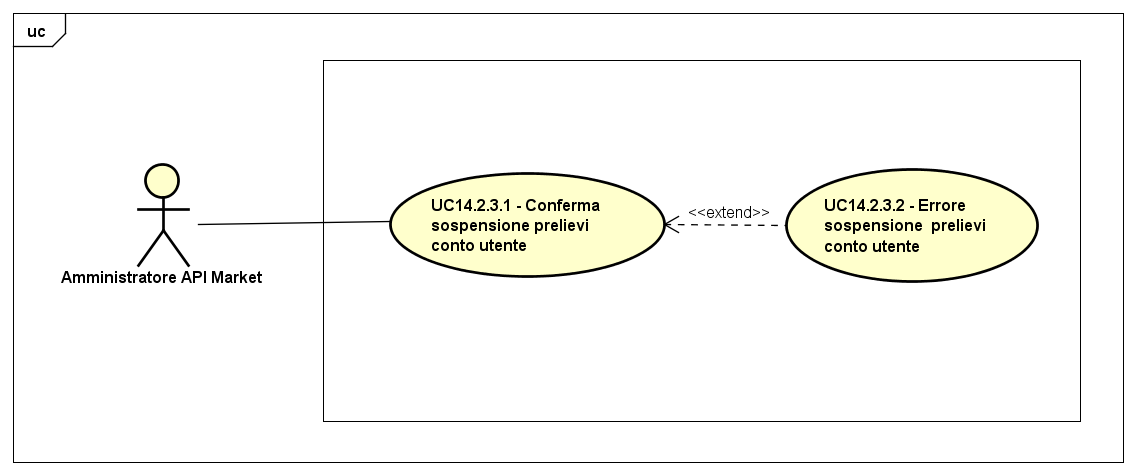
\includegraphics[scale=0.45]{UML/UC14_2_3.png}
	\caption{UC14.2.3: Sospensione prelievi conto utente}
\end{figure}

\begin{minipage}{\linewidth}
	\begin{tabular}{ l | p{11cm}}
		\hline
		\rowcolor{Gray}
		\multicolumn{2}{c}{UC14.2.3 - Sospensione prelievi conto utente} \\
		\hline
		\textbf{Attori} & Amministratore API Market \\
		\textbf{Descrizione} & L'attore sospende a tempo indeterminato i prelievi dell'utente scelto dal rispettivo conto personale \\
		\textbf{Pre-Condizioni} & L'attore si trova nella schermata relativa alla moderazione dell'utenza ed ha scelto un utente \\
		\textbf{Post-Condizioni} & L'attore ha sospeso a tempo indeterminato i prelievi dell'utente scelto dal rispettivo conto personale \\
		\textbf{Scenario Principale} & 
		\begin{enumerate*}[label=(\arabic*.),itemjoin={\newline}]
			\item L'attore può sospendere a tempo indeterminato i prelievi dell'utente scelto dal rispettivo conto personale
		\end{enumerate*}\\
		\textbf{Scenari Alternativi} & 
		\begin{enumerate*}[label=(\arabic*.),itemjoin={\newline}]
			\item L'attore può visualizzare un messaggio di errore informativo e la sospensione a tempo indeterminato dei prelievi dell'utente scelto dal rispettivo conto personale non avviene
		\end{enumerate*}\\
	\end{tabular}
\end{minipage}

\subparagraph{Caso d'uso UC14.2.3.1: Conferma sospensione prelievi conto utente}
\label{UC14_2_3_1}

\begin{minipage}{\linewidth}
	\begin{tabular}{ l | p{11cm}}
		\hline
		\rowcolor{Gray}
		\multicolumn{2}{c}{UC14.2.3.1 - Conferma sospensione prelievi conto utente} \\
		\hline
		\textbf{Attori} & Amministratore API Market \\
		\textbf{Descrizione} & L'attore conferma la sospensione a tempo indeterminato dei prelievi dell'utente scelto dal rispettivo conto e visualizza un messaggio di successo \\
		\textbf{Pre-Condizioni} & L'attore si trova nella schermata relativa alla moderazione dell'utenza ed ha scelto un utente \\
		\textbf{Post-Condizioni} & L'attore ha confermato la sospensione a tempo indeterminato dei prelievi dell'utente scelto dal rispettivo conto \\
		\textbf{Scenario Principale} & 
		\begin{enumerate*}[label=(\arabic*.),itemjoin={\newline}]
			\item L'attore conferma la sospensione a tempo indeterminato dei prelievi dell'utente scelto dal rispettivo conto e visualizza un messaggio di successo
		\end{enumerate*}\\
	\end{tabular}
\end{minipage}

\subparagraph{Caso d'uso UC14.2.3.2: Errore sospensione prelievi conto utente}
\label{UC14_2_3_2}

\begin{minipage}{\linewidth}
	\begin{tabular}{ l | p{11cm}}
		\hline
		\rowcolor{Gray}
		\multicolumn{2}{c}{UC13.2.3.2 - Errore sospensione prelievi conto utente} \\
		\hline
		\textbf{Attori} & Amministratore API Market \\
		\textbf{Descrizione} & L'attore visualizza un messaggio di errore informativo e la sospensione a tempo indeterminato dei prelievi dell'utente scelto dal rispettivo conto personale non avviene \\
		\textbf{Pre-Condizioni} & L'attore ha confermato la sospensione a tempo indeterminato dei prelievi dell'utente scelto dal rispettivo conto personale ma si è verificato un errore \\
		\textbf{Post-Condizioni} & L'attore ha visualizzato un messaggio di errore informativo \\
		\textbf{Scenario Principale} & 
		\begin{enumerate*}[label=(\arabic*.),itemjoin={\newline}]
			\item L'attore può visualizzare un messaggio di errore informativo e la sospensione a tempo indeterminato dei prelievi dell'utente scelto dal rispettivo conto personale non avviene
		\end{enumerate*}\\
	\end{tabular}
\end{minipage}

\paragraph{Caso d'uso UC14.2.4: Revoca sospensione utente}
\label{UC14_2_4}

\begin{minipage}{\linewidth}
	\begin{tabular}{ l | p{11cm}}
		\hline
		\rowcolor{Gray}
		\multicolumn{2}{c}{UC14.2.4 - Revoca sospensione utente} \\
		\hline
		\textbf{Attori} & Amministratore API Market \\
		\textbf{Descrizione} & L'attore revoca la sospensione dell'utente scelto, ricevendo un messaggio di successo \\
		\textbf{Pre-Condizioni} & L'attore si trova nella schermata relativa alla moderazione dell'utenza ed ha scelto un utente \\
		\textbf{Post-Condizioni} & L'attore ha revocato la sospensione dell'utente scelto, ricevendo un messaggio di successo \\
		\textbf{Scenario Principale} & 
		\begin{enumerate*}[label=(\arabic*.),itemjoin={\newline}]
			\item L'attore può revocare la sospensione dell'utente scelto, ricevendo un messaggio di successo
		\end{enumerate*}\\
	\end{tabular}
\end{minipage}

\paragraph{Caso d'uso UC14.2.5: Revoca sospensione prelievi conto utente}
\label{UC14_2_5}

\begin{minipage}{\linewidth}
	\begin{tabular}{ l | p{11cm}}
		\hline
		\rowcolor{Gray}
		\multicolumn{2}{c}{UC14.2.5 - Revoca sospensione prelievi conto utente} \\
		\hline
		\textbf{Attori} & Amministratore API Market \\
		\textbf{Descrizione} & L'attore revoca la sospensione dei prelievi dell'utente scelto dal rispettivo conto personale, ricevendo un messaggio di successo \\
		\textbf{Pre-Condizioni} & L'attore si trova nella schermata relativa alla moderazione dell'utenza ed ha scelto un utente \\
		\textbf{Post-Condizioni} & L'attore ha revocato la sospensione dei prelievi dell'utente scelto dal rispettivo conto personale, ricevendo un messaggio di successo \\
		\textbf{Scenario Principale} & 
		\begin{enumerate*}[label=(\arabic*.),itemjoin={\newline}]
			\item L'attore può revocare la sospensione dei prelievi dell'utente scelto dal rispettivo conto personale, ricevendo un messaggio di successo
		\end{enumerate*}\\
	\end{tabular}
\end{minipage}